\documentclass[a4paper,10pt, notitlepage]{report}
\usepackage[utf8]{inputenc}
\usepackage{natbib}
\usepackage{amssymb}
\usepackage{amsmath}
\usepackage{enumitem}
\usepackage{xcolor}
\usepackage{url}
\usepackage{cancel}
\usepackage{mathtools}
\usepackage[portuguese]{babel}
\usepackage{newclude}
\usepackage{booktabs}
\usepackage[normalem]{ulem}

%%%%%%%%%%%%%%%%%%%% Notation stuff
\newcommand{\pr}{\operatorname{Pr}} %% probability
\newcommand{\vr}{\operatorname{Var}} %% variance
\newcommand{\rs}{X_1, X_2, \ldots, X_n} %%  random sample
\newcommand{\irs}{X_1, X_2, \ldots} %% infinite random sample
\newcommand{\rsd}{x_1, x_2, \ldots, x_n} %%  random sample, realised
\newcommand{\bX}{\boldsymbol{X}} %%  random sample, contracted form (bold)
\newcommand{\bx}{\boldsymbol{x}} %%  random sample, realised, contracted form (bold)
\newcommand{\bT}{\boldsymbol{T}} %%  Statistic, vector form (bold)
\newcommand{\bt}{\boldsymbol{t}} %%  Statistic, realised, vector form (bold)
\newcommand{\emv}{\hat{\theta}}
\DeclarePairedDelimiter\ceil{\lceil}{\rceil}
\DeclarePairedDelimiter\floor{\lfloor}{\rfloor}
\DeclareMathOperator*{\argmax}{arg\,max}
\DeclareMathOperator*{\argmin}{arg\,min}
%%%%
\newif\ifanswers
\answerstrue % comment out to hide answers

% Title Page
\title{Primeira avaliação (A1)}
\author{Disciplina: Modelagem Estatística \\ Instrutor: Luiz Max Carvalho \\ Monitor: Isaque Pim}
\date{15 de Abril de 2023}

\begin{document}
\maketitle

\begin{center}
\fbox{\fbox{\parbox{1.0\textwidth}{\textsf{
    \begin{itemize}
        \item O tempo para realização da prova é de 3 horas;
        \item Leia a prova toda com calma antes de começar a responder;
        \item Responda todas as questões sucintamente;
        \item Marque a resposta final claramente com um quadrado, círculo ou figura geométrica de sua preferência;
        \item A prova vale 100 pontos. A pontuação restante é contada como bônus;
        \item Apenas tente resolver a questão bônus quando tiver resolvido todo o resto;
        \item Você tem direito a trazer \textbf{\underline{uma} folha de ``cola''} tamanho A4 frente e verso, que deverá ser entregue junto com as respostas da prova.
    \end{itemize}}
}}}
\end{center}

\newpage

\section*{1. Todo dia ela faz tudo sempre igual.}

Palmirinha se levanta todos dias às seis horas da manhã para ir ao estúdio gravar seus programas de culinária.
Preocupada com o trânsito, ela resolve documentar quanto tempo (em minutos) ela leva para chegar ao trabalho ($y$) dependendo da hora em que sai de casa, $x$, medida em `minutos depois das 6h'.
Os dados obtidos foram
\begin{table}[!h]
 \centering
\begin{tabular}{@{}|c|c|c|c|c|c|c|c|@{}}
\toprule
x & 0  & 10 & 20 & 30 & 40 & 50 & 60 \\ \midrule
y & 16 & 27 & 28 & 39 & 39 & 48 & 51 \\ \bottomrule
\end{tabular}
\end{table}

Muito esperta, Palmirinha logo ajusta uma regressão linear por mínimos quadrados, obtendo o seguinte gráfico:
\begin{figure}[!h]
    \centering
    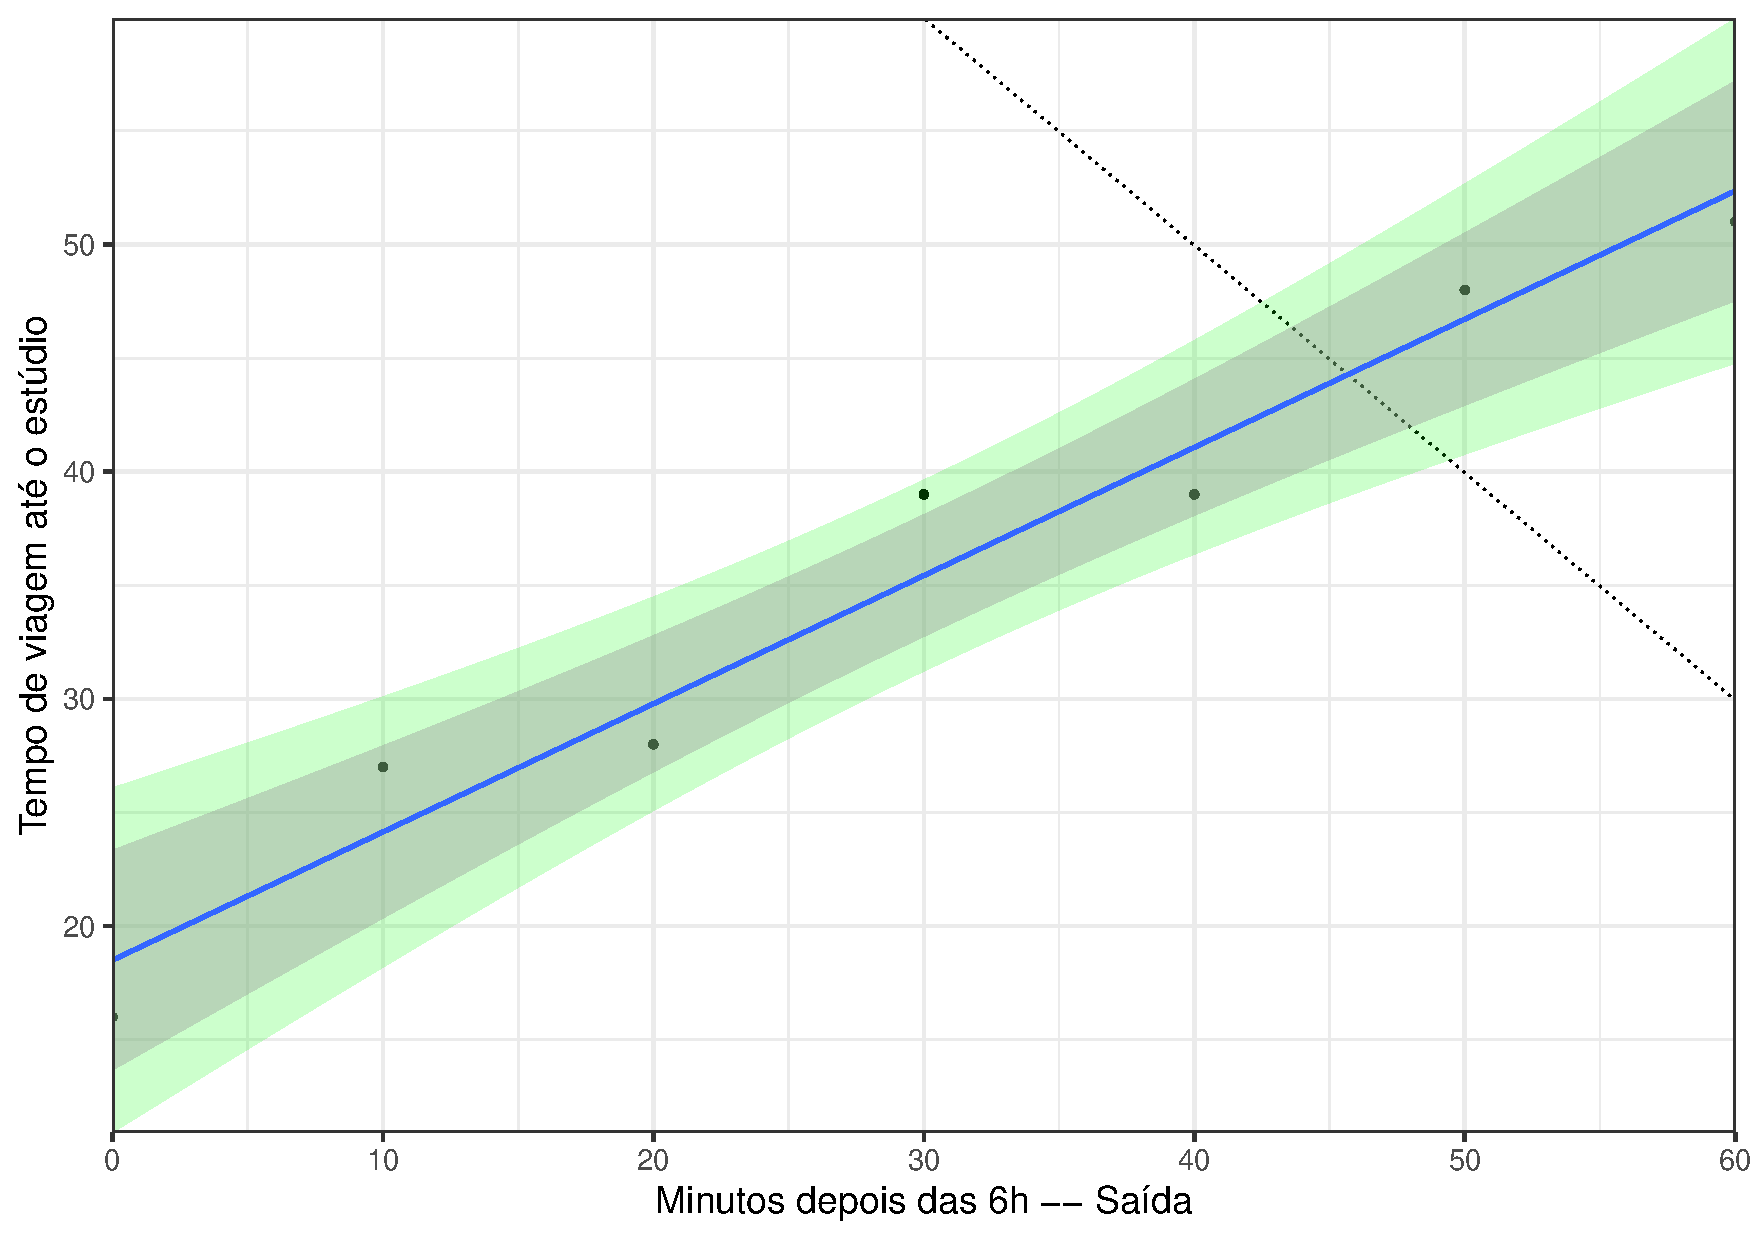
\includegraphics[scale=0.4]{scatter_palmirinha.pdf}
    \caption{Tempo de viagem até o estúdio de acordo com a hora da saída de casa.}
    \label{fig:my_label}
\end{figure}

\begin{enumerate}[label=\alph*)]
 \item (10 pontos) O neto de Palmirinha, Vítor Pereira, muito espevitado, olha os dados e exclama: ``Vovó, nem precisa estimar o intercepto! É só olhar os dados! O intercepto é 16.''.
  Vítor está errado, é claro.
  Mas porque será que ele pensa assim?
  Qual a estimativa correta do intercepto?
 \item (10 pontos) Palmirinha já foi avisada pela chefia de que não deve chegar depois das 7:30h.
 Mostre como ela pode determinar a hora máxima que pode sair de casa para que não chegue atrasada, em média.
 \item (10 pontos) Nossa heroína se preocupa que fazer seus cálculos tendo em vista a média do tempo de chegada e não o tempo de chegada em si pode criar problemas.
 Mostre à Palmirinha como determinar a hora de sair de casa para que ela chegue antes do horário limite com 99\%  de probabilidade.
 \item (20 pontos) Sendo uma bayesiana \textit{old school}, Palmirinha decide fazer um ajuste bayesiano do modelo linear aos dados apresentados.
 Como gosta de viver perigosamente, ela decide pela seguinte especificação de modelo e prioris:
 \begin{align*}
     y_i &= \beta_0 + \beta_1 x_i + \varepsilon_i,\\
     \varepsilon_i & \sim \operatorname{Normal}(0, \sigma^2),\\
     & \pi_B(\beta_0, \beta_1) \propto 1,\\
     & \pi_S(\sigma^2) \propto \frac{1}{\sigma^2},
 \end{align*}
 isto é, Palmirinha escolheu prioris \textbf{impróprias} para as quantidades desconhecidas do modelo.
 Calcule as esperanças \textit{a posteriori} $E_p[\beta_0 \mid \boldsymbol{y}; \boldsymbol{x}]$ e $E_p[\beta_1 \mid \boldsymbol{y}; \boldsymbol{x}]$ e discuta sua relação com os estimadores de mínimos quadrados obtidos anteriormente.
\end{enumerate}
\ifanswers
\include*{A1_2023_sol1}
\fi

\section*{2.  Facts and logi(sti)c } 
Um dos tipos mais comuns de dados são os dados binários, da forma $Y_i \in \{0, 1\}$.
Suponha que $\boldsymbol{X}$ é uma matriz $n \times P$ de covariáveis e $\boldsymbol{Y} = \{Y_1, \ldots, Y_n\}$ são observações binárias da variável dependente.
Para este tipo de dado, em geral estamos interessados em modelar a probabilidade $p_i := \pr(Y_i = 1; \boldsymbol{X}_i)$.
Considere o modelo
\begin{align*}
    Y_i &\sim \operatorname{Bernoulli}(p_i),\\
    p_i &:= \pr(Y_i = 1; \boldsymbol{X}_i) = \frac{\exp\left(\boldsymbol{X}_i^T\boldsymbol{\beta}\right)}{1 + \exp\left(\boldsymbol{X}_i^T\boldsymbol{\beta}\right)}.
\end{align*}

\begin{enumerate}[label=\alph*)] 
 \item (20 pontos) Mostre que a \textit{log chance} (em inglês, \textit{log-odds}) vale
 \begin{equation*}
     \log\left(\frac{\pr(Y_i = 1; \boldsymbol{X}_i)}{\pr(Y_i = 0; \boldsymbol{X}_i)}\right) = \boldsymbol{X}_i^T\boldsymbol{\beta}.
 \end{equation*}
  \item (20 pontos) Gostaríamos de obter estimativas $\hat{\boldsymbol{\beta}}$ para os coeficientes.
  Para tanto, podemos tentar maximizar a (log) verossimilhança dos dados observados sob o modelo em questão.
  No desenrolar dos cálculos no entanto, veremos que a equação 
  \begin{equation*}
      \nabla l(\boldsymbol{\beta}) = 0
  \end{equation*}
não tem solução em forma fechada.
Para encontrar a raiz -- isto é, o EMV $\hat{\boldsymbol{\beta}}$ -- precisamos de um método aproximado.
O Método de Newton-Raphson envolve fazer updates da forma
\begin{equation*}
    \boldsymbol{\beta}^{(t + 1)} = \boldsymbol{\beta}^{(t)} + \left[\boldsymbol{H}(\boldsymbol{\beta}^{(t)})\right]^{-1}\nabla l(\boldsymbol{\beta}^{(t)}),
\end{equation*}
para $t = 1, 2, \ldots$ a partir de um chute inicial $\boldsymbol{\beta}^{(0)}$.

Um critério de parada comum é 
\begin{equation*}
    \frac{||\boldsymbol{\beta}^{(t + 1)} - \boldsymbol{\beta}^{(t)} ||}{||\boldsymbol{\beta}^{(t)}||} \leq \varepsilon.
\end{equation*}
  \begin{enumerate}
      \item Calcule a log-verossimilhança em função de $\boldsymbol{\beta}$, bem como seu gradiente ($\nabla l(\boldsymbol{\beta}^{(t)})$) e matriz hessiana ($\boldsymbol{H}(\boldsymbol{\beta}^{(t)})$);
      
      \textbf{Dica}: Se quiser, pode considerar apenas um preditor mais o intercepto, isto é, $\boldsymbol{\beta} = (\beta_0, \beta_1)$.
      
      \item Argumente que a log-verossimilhança é estritamente côncava e que, portanto, o método de Newton-Raphson converge para um máximo global;
  \end{enumerate}
  \item (20 pontos) Suponha que queremos estudar a probabilidade de ter um ataque do coração: $Y_i = 1$ se o $i$-ésimo indivíduo sofreu um ataque do coração e $Y_i = 0$ caso contrário.
 Suponha ainda que  $X_j$ é uma covariável binária que codifica se o indivíduo torce para o Clube de Regatas do Flamengo (CRF): $X_{ij} = 1$ se o $i$-ésimo indivíduo torce para o CRF e $X_{ij} = 0$ caso contrário.
 Mostre como obter um \underline{intervalo de confiança} aproximado de 68\% para a razão de chance (\textit{odds ratio}), $\operatorname{OR}_j$:
 \begin{equation*}
     \operatorname{OR}_j = \frac{\pr(Y_i = 1; X_{ij} = 1)}{\pr(Y_i = 0; X_{ij} = 1)}  \bigg/\frac{\pr(Y_i = 1; X_{ij} = 0)}{\pr(Y_i = 0; X_{ij} = 0)}.
 \end{equation*}
 \textbf{Dica:} Expresse $\operatorname{OR}_j$ em função dos coeficientes e assuma que é possível obter uma estimativa do erro-padrão $\operatorname{se}_j$ para cada coeficiente.  
\end{enumerate} 
\ifanswers
\include*{A1_2023_sol2}
\fi

\section*{3. Found in translation}

Tome $\boldsymbol{Y}$ um vetor $n \times 1$ de variáveis dependentes com $Y_i \in \mathbb{R}$ e $\boldsymbol{X}$ uma matriz \textcolor{red}{\sout{$n \times P$ de covariáveis.}} \textcolor{blue}{$n \times (P+1)$ de  P covariáveis mais uma coluna de uns $X_0 = (1,1,\dots,1)^T$ representando o intercepto.} 
Considere a seguinte transformação das covariáveis:
\begin{equation*}
    Z_j = c_{j0} + \sum_{k=1} c_{jk}X_k,
\end{equation*}
formando a matriz $\boldsymbol{Z}$, que é $n \times (P + 1)$.

Agora suponha que vamos ajustar dois modelos de regressão linear múltipla:
\begin{enumerate}[label=\Roman*.]
    \item $\boldsymbol{Y} = \boldsymbol{X}^T \boldsymbol{\beta} + \boldsymbol{\varepsilon}$, onde $\boldsymbol{\varepsilon}$ é um vetor $n \times 1$ de erros independentes com  média $0$ e variância $\sigma^2$. 
    \item  $\boldsymbol{Y} = \boldsymbol{Z}^T \boldsymbol{\alpha} + \tilde{\boldsymbol{\varepsilon}}$, onde $\tilde{\boldsymbol{\varepsilon}}$ é um vetor $n \times 1$ de erros independentes com  média $0$ e variância $\tau^2$. 
\end{enumerate}

\begin{enumerate}[label=\alph*)]
 \item (10 pontos) Mostre que $\boldsymbol{Z}$  pode ser escrita como 
 \begin{equation*}
     \boldsymbol{Z} = \boldsymbol{X}\boldsymbol{t},
 \end{equation*}
 onde $\boldsymbol{t}$ é uma matriz $(P + 1) \times (P + 1)$.
 \item (10 pontos)  Mostre que a \textit{hat matrix} nos dois modelos é idêntica se $\boldsymbol{t}$ for inversível.
 \item (20 pontos) Mostre que se $\boldsymbol{t}$ for inversível, 
 \begin{equation*}
     \widehat{\boldsymbol{\alpha}} = \boldsymbol{t}^{-1}\widehat{\boldsymbol{\beta}},
 \end{equation*}
 onde $\hat{\boldsymbol{\beta}}$ é o estimador de mínimos quadrados de $\boldsymbol{\beta}$.
 Comente sobre o que esse resultado implica sobre a interpretação dos coeficientes sob transformações lineares da matriz de desenho.
 \end{enumerate}

\ifanswers
\include*{A1_2023_sol3}
\fi

% \bibliographystyle{apalike}
% \bibliography{refs}

\end{document}          
